\chapter{Implementacija}
\label{chap:implementacija}

Aplikacija je pisana u programskom jeziku Python verzije 2.7. Aplikacija se
dijeli u nekoliko zasebnih cjelina. U središtu aplikacije nalazi se cjovovod
koji poziva alate poput BLAST-a i fastacmd-a za komuniciranje sa NCBI-jevom
neredundantnom bazom, zatim dio aplikacije za odabir i balansiranje vrsta na
taksonomskom stablu te alat mafft\cite{mafft} za poravnanje sekvenci.  Pored cjevovoda
implementirana je web aplikacija kao korisničko sučelje za cijeli program. Web
aplikacija je implementirana koristeći Flask microframework, dok su operacije na
klijentskoj strani implementirane u javascriptu uz korištenje biblioteke jQuery.


\section{Cjevovod}
\label{sec:cjevovod}

Cjevovod je arhitektonski programski obrazac u kojem prolaze kroz filtre koji su
postavljeni jedan za drugim. Time se simulira jedan tok koji ulazne podatke
transformacijom kroz filtre generira izlazne podatke. U ovome projektu
cjevovodna arhitektura je samo logički kostur koji se enkapsulira unutar razreda
\emph{Pipeline}. Iako je u začetku razvoja aplikacije svaki filter bio zaseban
proces, vrlo ubrzo je ustanovljeno kako većina filtera generira podatke koji su
potrebni na raznim mjestima u cijeloj aplikaciji te se činilo lakše imati sve
podatke u memoriji pojedinog cjevovoda. To je omogućilo da razred
\emph{Pipeline} naslijedi razred \emph{Thread} iz modula \emph{threading} te se
može pozivati kao zasebna dretva.

Tok cjevovoda se može vidjeti na slici \ref{fig:cjevovod}. Ulaz u cjevovod
predstavljaju paralogni proteini u FASTA formatu koje zadaje korisnik. Ti se
podaci zadaju pri stvaranju objekta \emph{Pipeline} kako bi se mogli zapisati na
disk u direktorij vezan za instancu \emph{Pipeline-a}. Stvarni objekt kojeg
prima konstruktor \emph{Pipeline-a} je rječnik prilagođen uporabi web
aplikacije, što je detaljnije opisano u odjeljku \ref{sec:server}.

% SLIKA CJEVOVODA % TODO
\begin{figure}[h!]
\centering
%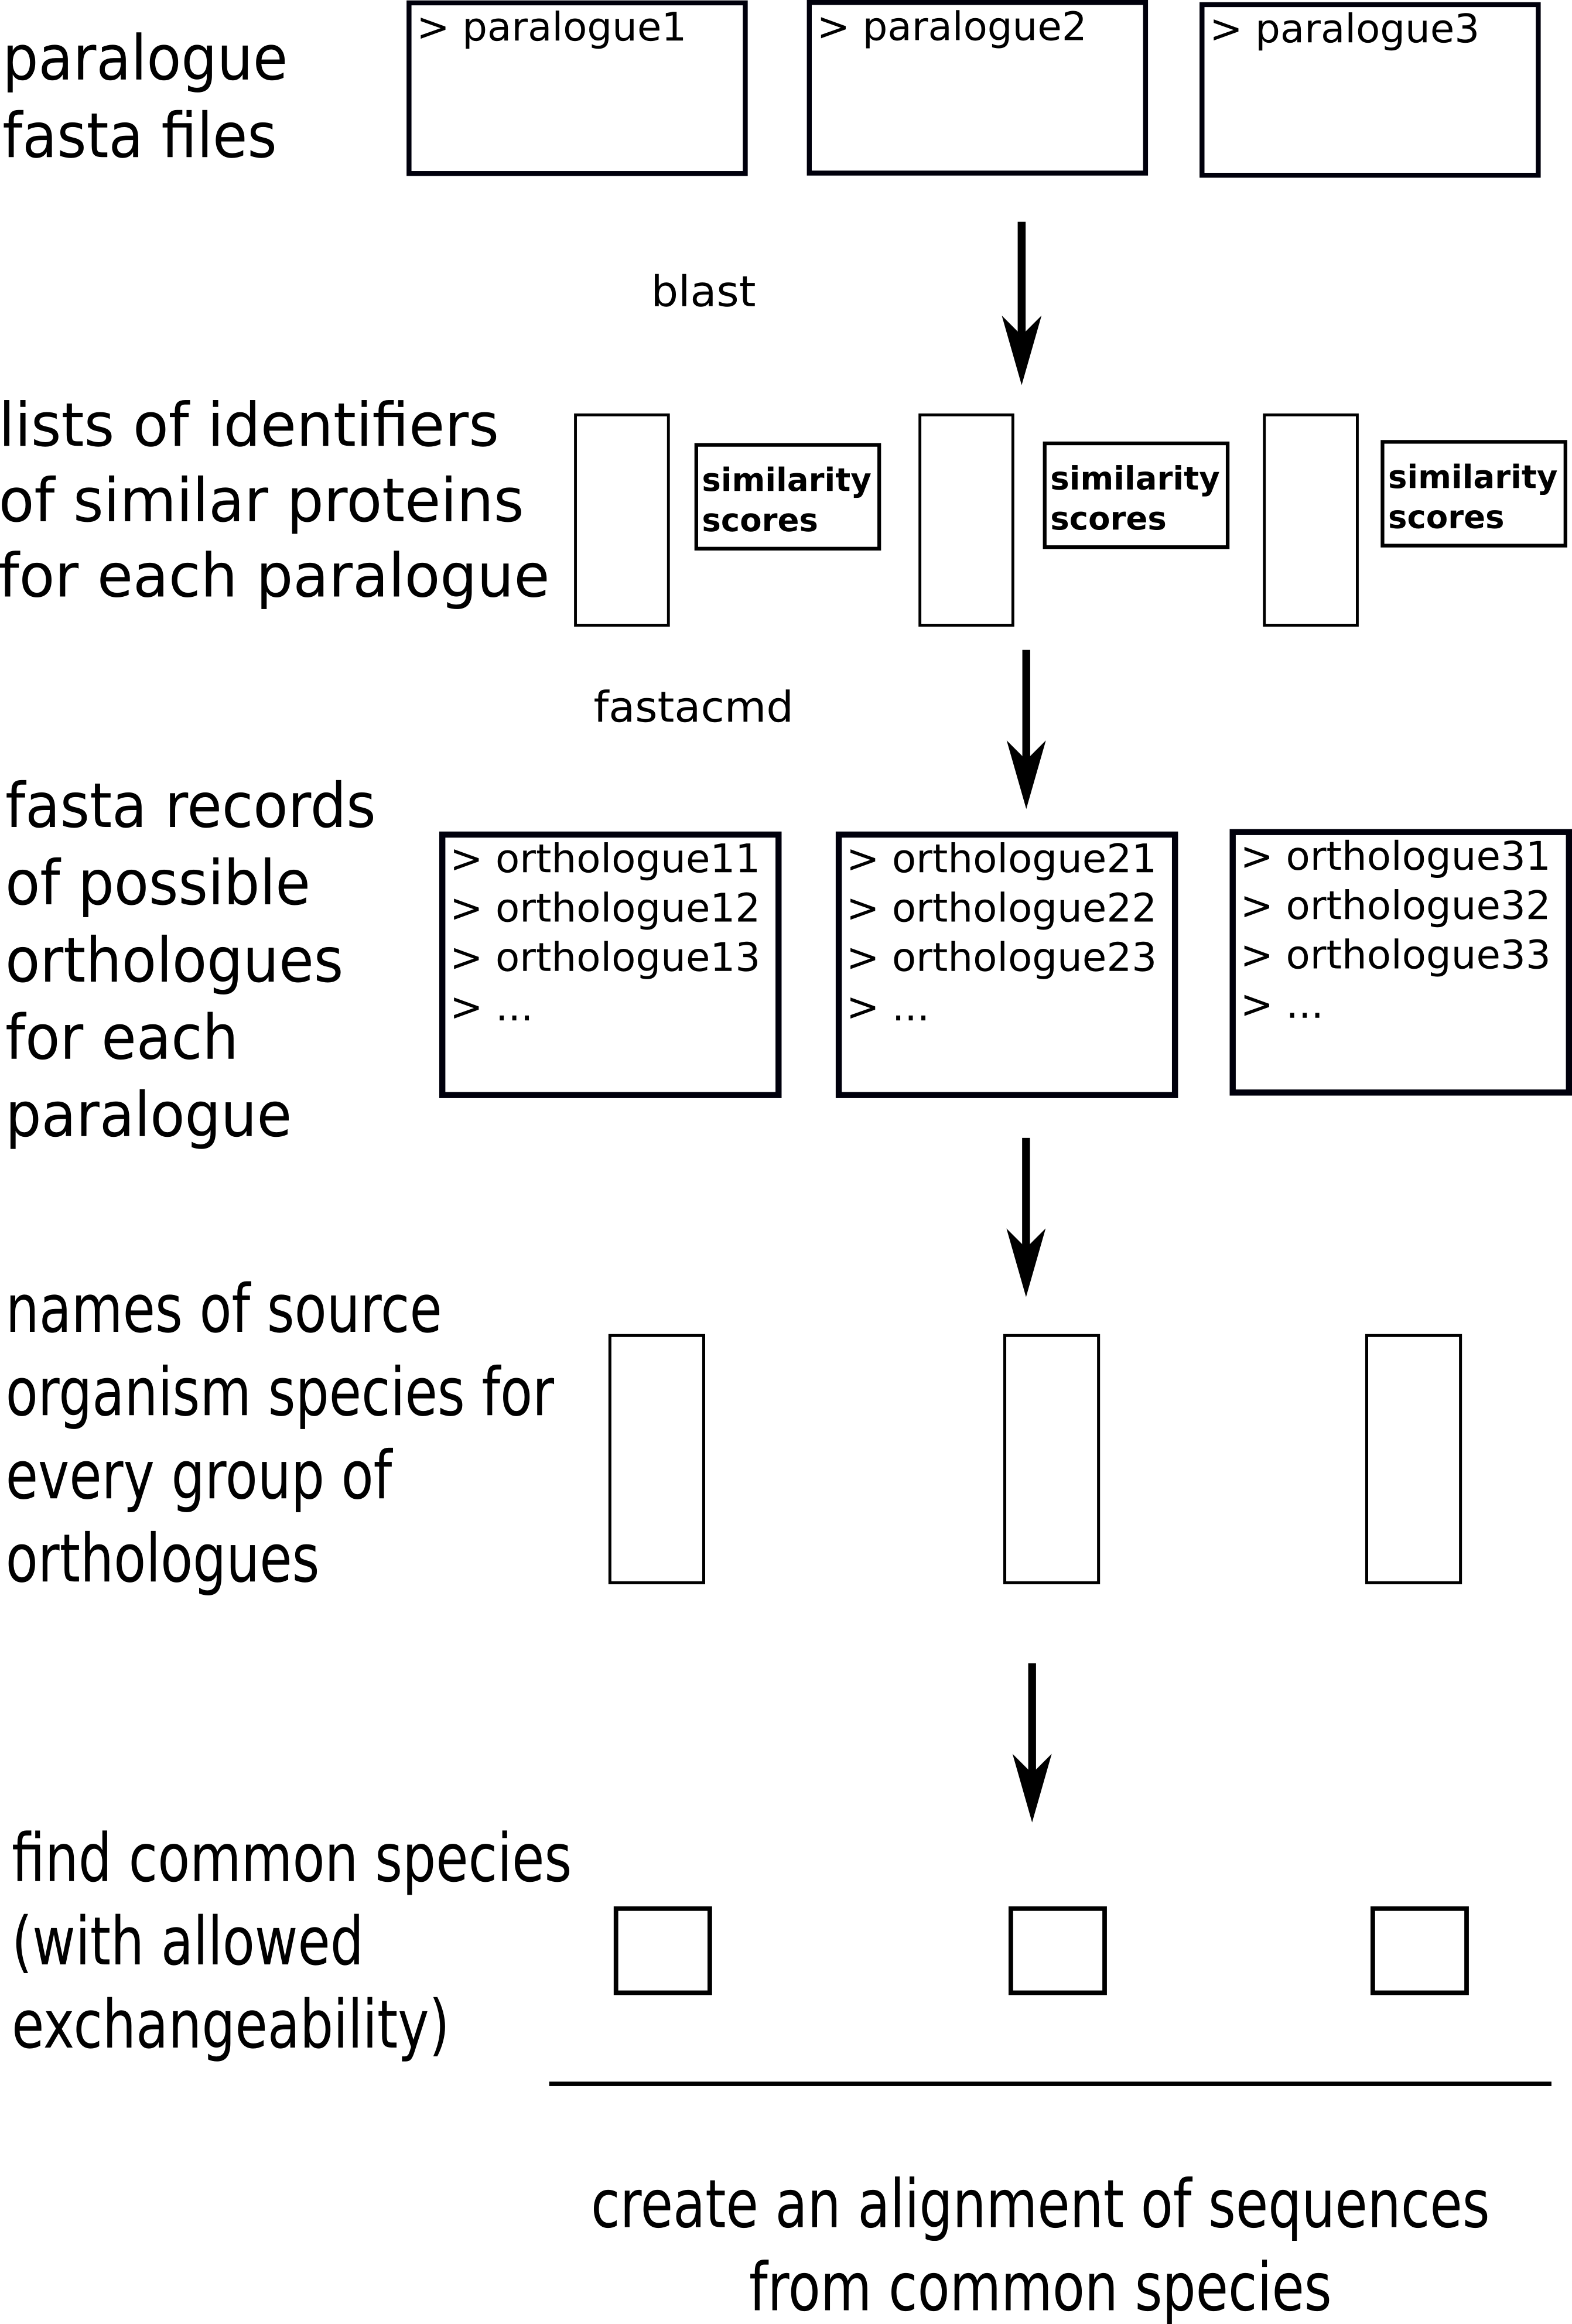
\includegraphics[width=1.0\linewidth]{figures/cjevovod.png}
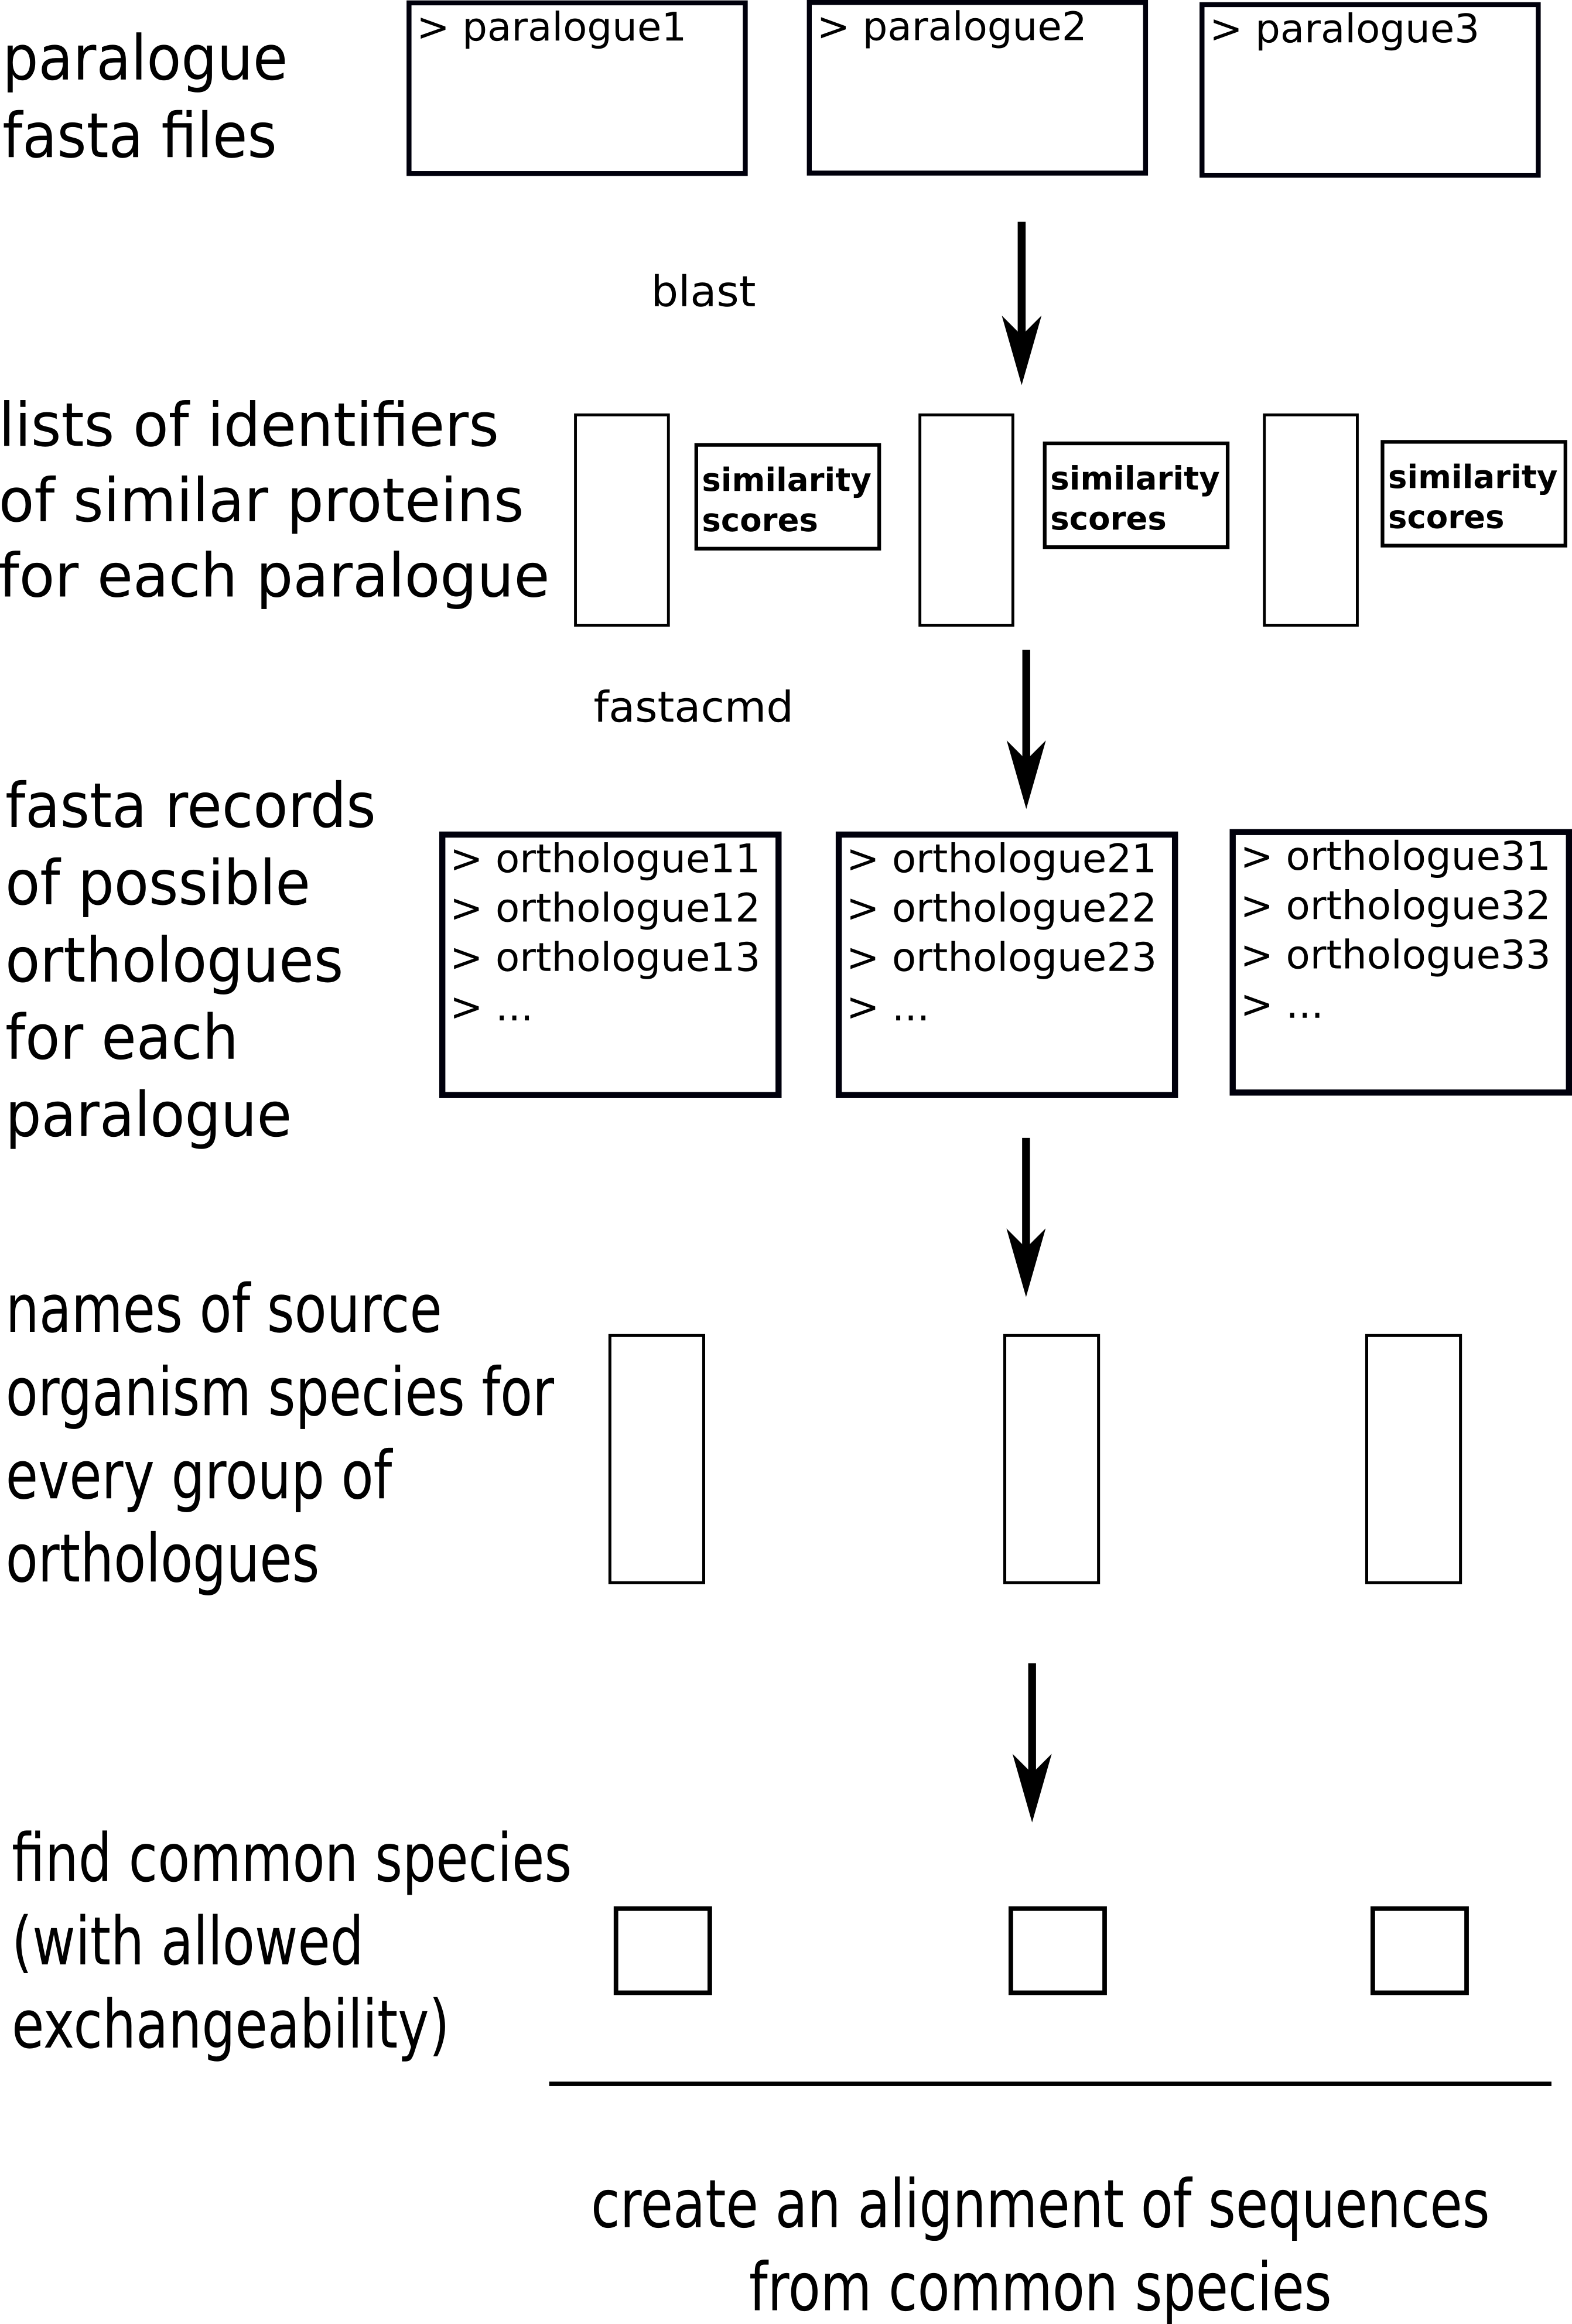
\includegraphics[width=4.5in]{figures/cjevovod.png}
\caption{Protok podataka kroz cjevovod. Prikazuju se podaci rađe nego filtri
radi boljeg uvida u rad cjevovoda}
\label{fig:cjevovod}
\end{figure}

Pri pokretanju cjevovoda za svaku se od unesenih sekvenci stvara objetk razreda
\emph{ProteinHolder} prilikom čega se obavljaju pozivi filtara nezavisnih za
svaku pojedinu sekvencu. Prvi filter koji se koristi je alat \emph{BLAST} te je
izveden kao poziv zasebnog izvršnog programa \emph{blastall} na sljedeći način:
\begin{lstlisting}[language=bash]
blastall -p blastp -i <ulaz-FASTA> -d <nr-baza> -m 8 -a <broj-dretvi>
\end{lstlisting}
Argument \emph{p} s parametrom \emph{blastp} označava programu da se koristi
algoritam za uspoređivanje jedne ulazne sekvence amino kiselina sa bazom
proteinskih sekvenci. S argumentom \emph{i} se zadaje put do ulazne datoteke s
FASTA sekvencom. Nadalje, argument \emph{d} prima put na disku do NCBI-jeve 
nereduntantne baze sekvenci koja je prethodno formatirana za pretraživanje
sekvenci u FASTA formatu. Argument \emph{m} određuje format ispisa koji generira
\emph{blastall}, a parametar 8 označava tabularni ispis bez dodatnih komentara
koji je pogodan za parsiranje. Konačno, argument \emph{a} upućuje
\emph{blastall} na broj dretvi koji treba koristiti kako bi se ubrzalo njegovo
izvođenje. Broj dretvi se u Orthobalanceru može postaviti prilikom instalacije.

Izlaz koji generira \emph{BLAST} predstavlja informacije o sekvencama sličnim
ulaznoj sekvenci, odnosno informacije o potencijalnim ortolozima za ulazni
paralog. Svaki redak, između ostalih, sadrži dvije bitne informacije:
jedinstveni ključ sekvence u neredundantnoj bazi --- gi-broj --- te ocjenu
sličnosti ulaznome paralogu. Nakon parsiranja tog izlaza ocjene sličnosti se
spremaju za kasniju upotrebu, a gi-brojevi se zapisuju u privremenu datoteku za
sljedeći korak u cjevovodu.

Sljedeći filter je izvršni program \emph{fastacmd} koji za svaki gi-broj pronalazi
i ispisuje sekvencu u FASTA formatu, također koristeći NCBI-jevu neredundantnu
bazu. Program se poziva ovako:
\begin{lstlisting}[language=bash]
fastacmd -i <ulaz> -d <nr-baza>
\end{lstlisting}
Budući da program \emph{fastacmd} dolazi u paketu zajedno sa \emph{BLAST}
alatima, argumenti imaju sličnu konotaciju kao i za \emph{blastall}: s
argumentom \emph{i} se zadaje ulazna datoteka, a s \emph{d} put do neredundantne
baze.

Izlaz \emph{fastacmd}-a se parsira pomoću razreda FastaRecord. Svaka dobivena
sekvenca kao kandidat za ortologa dobiva instancu razreda FastaRecord u kojoj je
sadržana sekvenca te sve bitne informacije iz zaglavlja pojedinog FASTA zapisa.
Dodatno, instanci FastaRecord se pridružuje ocjena sličnosti sekvence koju
opisuje prema ulaznom paralogu. Kako bi bilo lakše objasniti što je preuzeto iz
zaglavlja pojedinog FASTA zapisa, bitno je imati na umu strukturu neredundantne
baze što je objašnjenu u poglavlju \ref{chap:podaci}. Naime, ako je za nekoliko
proteina zabilježeno da imaju identičnu sekvencu, tada će zaglavlje takve FASTA
sekvence u neredundantnoj bazi sadržavati spojene podatke o navedenim
proteinima. 
Zato objekt razreda FastaRecord sadrži listu elemenata zaglavlja,
gdje se svaki od tih elemenata opisuje n-torkom (gi-broj elementa, ime vrste, ime
proteina, zastavica: najbolja sekvenca za ovaj gi-broj). Iako je poznato
da neredundantna baza sadrži sekvence sakupljene iz raznih baza što implicira
činjenicu da zaglavlja pojedinih sekvenci ne moraju imati identičan oblik,
uočeno je određeno pravilo po kojem \emph{fastacmd} ispisuje sekvence te se ono
koristi kao heuristika ugrađena u parser. Pretpostavljeni oblik pojedinog
elementa zaglavlja je sljedeći:\\
\texttt{>gi|"gi-broj"|nebitne-informacije IME PROTEINA}\\
\texttt{[IME VRSTE]nebitna-informacija}.\\
Na primjer:\\
\texttt{>gi|\textbf{344243907}|gb|EGW00011.1| \textbf{Cofilin-1}
[\textbf{Cricetulus griseus}]}\\

Na kraju obrade podataka za pojedini paralog s ulaza prolazi se listom svih
objekata FastaRecord te se za svaku pronađenu vrstu odabire sekvenca s najboljom
ocjenom sličnosti. Time nastaje jedan podskup sekvenci za koje možemo reći da
predstavljaju grupu ortologa za dani paralog.

Nakon što je svaki paralog opisan jednim objektom razreda \emph{ProteinHolder}
potrebno je odrediti postoji li koji gi-broj koji se može pronaći u grupama
ortologa različitih paraloga. Donesena je odluka kako to svojstvo nije poželjno
jer jedan te isti protein ne želimo imati kao predstavnika neke vrste u
različitim grupama ortologa. Za potrebe ove funkcionalnosti dodani su razredi
\emph{BestScore} i \emph{BestScoreCollection}. Razred \emph{BestScore} sadrži
informaciju koja upućuje u kojoj se grupi ortologa, na kojem FASTA zapisu te sa
kojim elementom zaglavlja FASTA zapisa nalazi najbolje ocijenjena sekvenca za
dani gi-broj identifikator. Razred \emph{BestScoreCollection} služi kao sučelje
za korištenje rječnika najboljih sekvenci, a nudi metode za ažuriranje rječnika
kandidatima za najbolje sekvence te metodu za dohvat trenutno postavljene
najbolje instance razreda \emph{BestScore}. Skica algoritma za pronalazak
najbolje ocijenjenih dana je algoritmom \ref{algo:best-score}. Nakon provedbe
algoritma nepoželjni proteini imaju spuštenu zastavicu najbolje sekvence za svoj
gi-broj te se ne razmatraju u nastavku programa.

\begin{algorithm}[h!]
\centering
\caption{Nalaženje najbolje ocijenjenih proteina}
\label{algo:best-score}
\begin{algorithmic}[1]
\Function{ProteinHolder::izračunajNajOcjene}{}
    \State $ocjene \gets BestScoreCollection()$
    \ForAll{$fastaRecord \in this.records$}
        \ForAll{$element \in fastaRecord.elementiZaglavlja$}
            \State $ocjena \gets BestScore(element)$
            \State $ocjene.ažuriraj(ocjena, fastaRecord.ocjena)$
        \EndFor
    \EndFor        
    \Return $ocjene$
\EndFunction

\Function{ProteinHolder::propagiraj}{$najOcjene$}
    \ForAll{$fastaRecord \in this.records$}
        \ForAll{$element \in fastaRecord.elementiZaglavlja$}
            \State $najOcjena \gets najOcjene.dohvati( element['gid'] )$
            \If{$\lnot najOcjena.provjeriElement( element )$}
                \State $element['zastavicaNajbolji'] \gets \bot$%\textbf{false}
            \EndIf
        \EndFor
    \EndFor
\EndFunction

\Function{pronađiNajOcjene}{$proteinHolders$}
\Comment{funkcija je isječak iz cjevovoda}
    \State $najOcjene \gets new BestScoreCollection()$
    \ForAll{$protein \in proteinHolders$}
        \State $ocjene \gets protein.izračunajNajOcjene()$
        \State $najOcjene.ažurirajKolekcijom( ocjene )$
    \EndFor
    \ForAll{$protein \in proteinHolders$}
    \Comment{propagacija najboljih ocjena}
        \State $protein.propagiraj(najOcjene)$
    \EndFor
\EndFunction
\end{algorithmic}
\end{algorithm}


Ovdje bi se još mogla dodati funkcionalnost kojom bi se za vrstu kojoj je
protein odbačen pronašao sljedeći najbolji nezauzeti protein, no to nije
razmatrano. Za takve slučajeve ne može se sa sigurnošču reći jesu li kodirajući
geni doista ortologni ili se u nekoj roditeljskoj vrsti gen duplicirao te se sa
takvim nejednoznačnostima aplikacija ne bavi.

Najbitniji korak u cjevovodu je pronalaženje i balansiranje zajedničkih vrsta na
stablu taksonomije živog svijeta. Ovaj korak je detaljno opisan u odjeljku
\ref{sec:tax}. Ovom se filtru kao ulaz predaju kompletni opisnici proteina,
odnosno objekti razreda \emph{ProteinHolder} iz kojih sam filter povlači sve
potrebne informacije. Nakon što završi obrada, izlaz filtra je predočen
višeslojnim rječnikom koji razdvaja podatke po sljedećim slojevima: grupe
ortologa, grupe zamjenskih čvorova u taksonomskom stablu, grupe balansiranih
čvorova u taksonomskom stablu te su zadnje vrijednosti balansirane vrste.

Zadnji korak u cjevovodu prije zapisivanja svih skupljenih podataka na disk je
poravnanje sekvenci dobivenih kao izlaz programa \emph{fastacmd}. Za poravnanje
se koristi alat \emph{mafft}\cite{mafft} te mu je ulaz datoteka sa zapisanim sekvencama u FASTA
formatu, a izlaz datoteka sa istim, ali poravnatim sekvencama. \emph{mafft} se
poziva na sljedeći način:
\begin{lstlisting}[language=bash]
mafft --auto <ulaz> > <izlaz>
\end{lstlisting} 
Argument --auto upućuje \emph{mafft} da automatski odabere najbolju strategiju
poravnavanja sekvenci, uzimajući u obzir veličinu podataka. Izlaz se direktno
preusmjerava u novu datoteku na disk jer poravnate sekvence nisu potrebne u
memoriji.

% TODO tekst o objetkima

% TODO SLIKA objekata (class dijagram)


\section{Nalaženje zajedničkih vrsta}
\label{sec:tax}

% TODO pomaknut ovo u uvod negdje; sredit citate
Pronalazak zajedničkih vrsta najbitniji je modul Orthobalancera. U suštini, ovaj
modul nije logički vezan za nalaženje ortologa, no za potrebe Ortobalancera je
svojim sučeljima prilagođen njegovom cjevovodu. Nalaženje zajedničkih vrsta među
skupovima ulaznih vrsta predstavlja jednu novu dimenziju u pronalasku ortolognih
proteina. Konvencionalno traženja ortologa\cite{Tatusov, Baratham} jest
kvalitetnije jer se pretraživanje odvija na razini sekvence, ali je moguće samo
za genome koji su u potpunosti istraženi i zapisani u baze
podataka.\cite{Flicek} Podizanje potrage za ortolozima na razinu vrsta omogućava
da se ortolozi pronađu i među vrstama čiji genomi nisu još zabilježeni.

Ovaj modul za svoj rad koristi podatke iz NCBI-jeve \emph{Taxonomy} baze.
Koristi se čvorovi taksonomskog stabla živog svijeta i znanstvena imena
pridijeljena čvorovima. Čvorovi su identificirani svojim jedinstvenim
identifikatorima \emph{tax\_id}, a svaki čvor ima pridruženo jedno ili više
korištenih imena. Samo jedno od tih imena je označeno kao znanstveno i također
je jedinstveno za svaki čvor, uz neke iznimke poput sintetički stvorenih vrsta
koje dijele znanstveno ime \emph{Synthetic construct}. Datoteke koje sadrže
podatke iz ovih baza su prilično velike te njihovo učitavanje, prilagođavanje i
korištenje najviše utječe na trajanje izvođenja programa.

Na početku rada modula svi podaci se prilagođavaju za potrebe modula. Iz
cjevovoda se od svake instance \emph{ProteinHolder}-a uzimaju zabilježene vrste,
a iz popisa zamjenjivih čvorova koje zadaje korisnik se prikupljaju svi zadani
čvorovi. Svim prikupljenim imenima se tada pridružuje \emph{tax\_id} iz baze.

Nakon toga se gradi taksonomsko stablo u memoriji. Stablo je izvedeno kao veliki
rječnik kojem za ključeve koristi \emph{tax\_id}, a svaki čvor je objekt razreda
\emph{Node}. Razred \emph{Node} sadrži sljedeće bitne podatke: \emph{tax\_id}
roditeljskog čvora, listu djece, brojač za svaku grupu ortologa, ukupni brojač
grupa, listu zamjenskih roditeljskih čvorova te zastavicu je li balansiran.
Brojači se inicijaliziraju na nulu, a kasnije tijekom algoritma će koristiti kao
broj vrsta pojedine grupe ortologa koje se nalaze pod danim čvorom. Ukupni
brojač grupa govori koliko ortolognih grupa ima svoga predstavnika pod nekim
čvorom. Lista zamjenskih roditeljskih čvorova se inicijalizira na praznu listu,
a bit će popunjena svim čvorovima koji su od korisnika označeni kao zamjenski te
se nalaze iznad trenutno razmatranog čvora. Zastavica za balansiranje koristi se
kasnije tijekom postupka balansiranja podstabala ispod zamjenskih čvorova.
Algoritam je opisan u nastavku, a dan je i njegov pseudokod \ref{algo:balance}.

Sljedeći koraci predstavljaju inicijalizaciju stabla. Najprije se za svaku
ortolognu grupu prolazi kroz sve vrste. Za svaku vrstu pronalazi se njen čvor,
odnosno list u stablu. Brojač tog lista za trenutnu ortolognu grupu se
inicijalizira na $1$. Istovremeno se ukupni brojač grupa u tome listu postavi na
$1$ te se pozove metoda koja propagira ukupni brojač grupa sve do korijena
stabla, pazeći da ukupni brojač niti u jednom čvoru ne bude više od jednom
povećan za neku grupu ortologa.
% TODO možda napisati pseudokod

Nakon toga treba inicijalizirati zamjenske čvorove i pripadna podstabla. Za
svaki zamjenski čvor poziva se rekurzivna funkcija koja se spušta do listova i
svakome čvoru u njegovu listu zamjenskih roditeljskih čvorova dodaje
\emph{tax\_id} zamjenskog čvora nad kojim je rekurzija pozvana.  Time svaki čvor
sadrži informaciju kojim zamjenskim podstablima pripada.

\begin{algorithm}[h!]

\centering
\caption{Obilazak stabla --- balansiranje vrsta}
\label{algo:balance}

\begin{algorithmic}[1]

\Require korijenski čvor stabla; $n$ skupova vrsta
\Ensure višeslojni rječnik $izlaz$ koji za svaki balansirani čvor sadrži
listu vrsta predstavnica iz svake grupe $g$  

\State \Comment algoritam obilaska počinje funkcijom $obidiStablo()$

\Function{balansiraj}{cvor, grupe}
    \State $izlaz \gets$ new $izlaz$
    \ForAll{$dijete \in cvor.djeca$}
        %\State $izlaz \gets izlaz \cup balansiraj(dijete, grupe)$
        \State $izlaz \gets izlaz$ $\cup$ \Call{balansiraj}{$dijete, grupe$}
        \If{$\neg dijete.balansiran$}
            \ForAll{$g \in grupe$}
                \State $cvor.brojac[g] \gets cvor.brojac[g] + dijete.brojac[g]$
            \EndFor
        \EndIf
    \EndFor
    \If{$cvor.brojac[g] > 0$ $\forall g \in grupe$}
        \State $cvor.balansiran \gets \textbf{istina}$
        \If{$\exists k \forall g \in grupe (cvor.brojac[g] = k)$}
        %\If{$\forall g \in grupe cvor.brojac[g] SU JEDNAKI$}
            \State $A \gets$ skup svih pripadajućih vrsta pod cvorom $cvor$
            \State $izlaz.pridruzi(A)$
        \Else
            \State $n \gets \min\{brojac[g] \in cvor\}$
            \State $R \gets \forall g \in grupe$ odaberi $n$ slučajnih vrsta pod
cvorom $cvor$
            \State $izlaz.pridruzi(R)$
        \EndIf
    \EndIf
    \State \Return $izlaz$
\EndFunction

% ovo zakomentirano sluzi za razbijanje algoritma na vise dijelova kako bi mogli
% biti prikazani na vise stranica u pdf-u
%\algstore{balans}
%\end{algorithmic}
%\end{algorithm}
%
%\begin{algorithm}[h!]
%\begin{algorithmic}[1]
%\algrestore{balans}

\Function{obidiStablo}{$cvor, grupe$}
    \If{$cvor.zamjenski()$}
    \Comment{vraća \textbf{istina} ako je čvor u zamjenskom podstablu}
        %\State \Return $balansiraj(cvor, grupe)$
        \State \Return \Call{balansiraj}{$cvor, grupe$}
    \Else
        \If{$cvor.list()$}
        \Comment{vraća \textbf{istina} ako je čvor list}
            \ForAll{$g\in grupe$}
                \State $izlaz[g][$'nezamjenski'$] \gets cvor.ime$
            \EndFor
        \Else
            \State $izlaz \gets$ new $izlaz$
            \ForAll{$dijete \in cvor.djeca$}
                \If{$dijete.ukupniBrojac = cvor.ukupniBrojac$}
                    %\State $izlaz \gets izlaz \cup obidiStablo(dijete, grupe)$
                    \State $izlaz \gets izlaz$ $\cup$ \Call{obidiStablo}{$dijete,
grupe$}
                \EndIf
            \EndFor
        \EndIf
    \EndIf
    \State \Return $izlaz$
\EndFunction

\end{algorithmic}
\end{algorithm}  


Slijedi algoritam \ref{algo:balance}. Algoritam rekurzivno prolazi stablom,
polazeći od listova. U zamjenskim podstablima balansira grupe ortologa na
sljedeći način. Nakon što se obiđu listovi, svaki čvor, za svaku od grupa
ortologa, postavlja svoj brojač za tu grupu na vrijednost zbroja brojača svoje
djece, pri čemu se od djece ne razmatraju već balansirani čvorovi. U slučaju da
nijedan brojač u čvoru ne ostane na vrijednosti $0$, čvor se proglašava
balansiran. Drugim riječima, u svakoj grupi ortologa postoji barem jedna vrsta
ispod toga čvora te se one mougu ispisati kao uparene ili zamjenjive vrste.  U
idealnom, ali i najčešćem slučaju, desit će se da je vrsta prisutna u svim
grupama ortologa te će tada sam čvor promatrane vrste biti proglašen
balansiranim i roditelji ga zbog oga neće razmatrati. Za primjenu nalaženja
ortolognih proteina to bi značilo da neka vrsta, na primjer Homo sapiens, sadrži
ortologni protein svakome od ulaznih paraloga. Algoritam je tako osmišljen kako
bi se balansirale što srodnije vrste.  Što se tiče dijelova stabla koji nisu pod
niti jednim zamjenskim čvorom, algoritam ne provodi postupak balansiranja te se
u izlaz dodaju jedino one vrste koje su prisutne u svim grupama ortologa. Izlaz
ovog algoritma vraća se pozivatelju, odnosno cjevovodu.


\section{Web aplikacija}
\label{sec:server}

Korisničko sučelje Orthobalancera ostvareno je kao web aplikacija implementirana
također u Pythonu koristeći Flask microframework. Flask je izgrađen na Werkzeug
WSGI\footnote{Web Server Gateway Interface\cite{pep333}} web alatu i Jinja2
sustavu predložaka. Flask je zvan \emph{microframeworkom} jer svoju jezgru drži
jednostavnom, ali proširivom. Flask također nudi određene konvencije koje
pojednostavljuju izgradnju web aplikacije. Osim Flaska, za razvoj aplikacije
korišten je javascript uz većinu koda napisanu pomoću biblioteke jQuery. Osim za
asinkronu komunikaciju s poslužiteljem pomoću AJAX-a\footnote{Asynchronous
JavaScript and XML}, javasvript se najviše koristio za postizanje dinamike te
robusnosti provjere i sinkronizacije ulaznih podataka.

% pomalo o svakom bitnom url-u / templatu
HTML\footnote{HyperText Markup Language} stranice koje aplikacija generira
bazirane su na Jinja2 predlošcima. Jedno od njihovih pogodnih svojstava je
nasljeđivanje predložaka. Time se omogućuje da postoji jedan temeljni predložak
koji sadrži osnovne elemente svake stranice, a ostali samo nasljeđuju te
elemente i popunjavaju potrebni sadržaj. HTML predlošci Orthobalancera su
sljedeći:

\begin{itemize}

    \item \emph{layout.html} definira raspored svih elemenata te ga svi ostali
predlošci nasljeđuju.

    \item \emph{input.html} prihvaća ulazne podatke od korisnika. Detaljniji
opis mogućnosti koje su ostvarene za ulazne podatke se nalazi u odjeljku.
\ref{sec:input}

    \item \emph{manipulate\_exchangeable.html} je stranica koja se prikazuje
samo kada korisnik želi unijeti vlastite zamjenske čvorove taksonomskog stabla.
Stranica se otvara s ponuđenim pretpostavljenim skupom zamjenskih čvorova.

    \item \emph{execution.html}  prikazuje trenutno stanje izvođenja, asinkrono
komunicirajući sa poslužiteljem, kako bi korisnik imao jasniju predodžbu o
zadacima koje poslužitelj obavlja te o trajanju izvođenja. Jednom kada stranica
za ispis primi poruku o kraju izvođenja, automatski se preusmjerava na URL
\textbf{'/output'}.

    \item \emph{output.html} prikazuje izlaz aplikacije korisniku. Prikazani
izlaz je tablica na slici \ref{fig:tablica}. Osim tablice, nude se poveznice na
niz datoteka za preuzimanje. Izlazne datoteke su opisane u odjeljku
\ref{sec:output}.

    \item \emph{error.html} se prikazuje ukoliko na poslužitelju dođe do
pogreške.

\end{itemize}

Poslužitelj Orthobalancera se može zamisliti kao stroj stanja kojemu su stanja
predočena URL-om\footnote{unified resource locator}. Flask radi tako da veže
URL na jednu funkciju Pythona\footnote{\emph{view} funkcija} koristeći
mehanizam dekoriranja\cite{pep} funkcije kojeg nudi Python. Na taj se način uz
svaki URL veže određeni posao koji treba obaviti. Bitniji URL-ovi su sljedeći:

\begin{itemize}

    \item \textbf{'/'} ulazna točka za pokretanje novog upita. Upit dobiva
jedinstveni identifikacijski broj te se za njega inicijaliziraju određeni podaci
na poslužitelju kao sjednički podaci. Automatski se preusmjerava na
\textbf{/start}. Od ove točke na dalje svaki URL ima identifikacijski broj upita
u svome parametru, što nije posebno naznačeno. Takav je način prenošenja
identifikacijskog broja odabran kako bi korisnik samo pomoću URL-a mogao
dohvatiti svoje rezultate.

    \item \textbf{'/start'} pozvan za inicijalizirani upit. Generira i vraća
HTML stranicu baziranu na predlošku \emph{input.html}.

    \item \textbf{'/finish\_input'} poziva se tek u trenutku kad su na klijentskoj
strani svi ulazni podaci pravilno uneseni. Podaci su tada već spremljeni u
sjedničkim varijablama te se može stvoriti instanca razreda \emph{Pipeline},
odnosno nova dretva cjevovoda. Ovisno o korisnikovom odabiru na stranici
\emph{input.html}, sljedeće stanje izvođenja može biti na URL-u
\textbf{'/get\_exchangeable'} ako korisnik želi zadati svoje zamjenske čvorove,
odnosno na URL-u \textbf{'/preparations'} za pokretanje cjevovoda s predloženim
zamjenskim čvorovima.

    \item \textbf{'/preparations'} čita sadržaj datoteke sa predloženim
zamjenskim čvorovima, sprema ih u argumente sjednice te se preusmjerava na URL
\textbf{'/executing'}.

    \item \textbf{'/get\_exchangeable'} generira stranicu baziranu na predlošku
\emph{manipulate\_exchangeable.html} s podacima  iz datoteke s predloženim
zamjenskim čvorovima.

    \item \textbf{'/save\_exchangeable'} sprema korisnikove zamjenske čvorove u
argumente sjednice te se preusmjerava na URL \textbf{'/executing'}.

    \item \textbf{'/executing'} pokreće rad dretve cjevovoda te generira
stranicu baziranu na predlošku \emph{execution.html}.

    \item \textbf{'/output'} generira stranicu iz predloška \emph{output.html}
predajući joj sve potrebne informacije dohvaćene iz datoteka koje je stvorio
izlaz cjevovoda.

\end{itemize}

% todo možda neki opis job/session (pitat Mile/Ivanu)
    
% LOG - možda posebna sekcija - todo pitat
Vrijeme izvođenja posla u cjevovodu može potrajati nekoliko minuta te je zato
bilo potrebno osmisliti način kako predočiti korisniku napredak izvođenja u
nekom trenutku. Rješenje je osmišljeno na način da cjevovod svoj napredak
zapisuje u \emph{log} datoteke, a klijent asinkrono traži od poslužitelja
sadržaj tih datoteka svakih nekoliko sekundi. Za odvajanje funkcionalnosti
ispisa stanja cjevovoda u \emph{log} datoteke iskorišten je Pythonov mehanizam
dekoriranja funkcija. Implementirani su razredi \emph{beforeMessage} i
\emph{afterMessage} koji imaju funkcionalnost dekoratora. Oba dekoratora imaju
argument --- ključ rječnika koji sadrži konkretan tekst za ispis u \emph{log}
datoteke. \emph{beforeMessage} dekorira funkciju tako da obavlja ispis prije
poziva dekorirane funkcije, a \emph{afterMessage} nakon izvršavanja dekorirane
funkcije. Oba razreda dekoratora nasljeđuju temeljni dekorator
\emph{messagingDecorators} koji sadrži implementaciju samog zapisivanja statusa
u \emph{log} datoteke, a izvedeni razredi se samo brinu o načinu dekoriranja.

% todo upute u sidebaru (možda nije potrebno - pitat)


\section{sinkronizacija ulaza}
\label{sec:input}

%ideja i srž implementacije sinkronizacije i ROBUSNOSTI unosa podataka slika

Jedan od nužnih preduvjeta za uspješan rad aplikacije jest pažljivo preuzimanje
ulaznih podataka uz robusne provjere. S druge strane bitno je omogućiti
raznolike načine unošenja podataka za lakše rukovanje aplikacijom. Orthobalancer
na ulazu očekuje dvije ili više proteinskih sekvenci od kojih će svaka
sadržavati različito ime. Elemente za unos podataka pojedinog proteina na
stranici moguće je dodavati dinamički. Sam FASTA zapis se može izravno upisati u
površinu za unos teksta, ili se može predati datoteka sa sadržajem FASTA zapisa.

Inicijalna ideja bila je sve provjere implementirati na strani klijenta pomoću
javascripta, no budući da javascript nije pogodan za otvaranje i čitanje
sadržaja datoteka odlučeno je da se podaci čuvaju na poslužitelju. Zbog toga je
potrebno prilikom svake promjene sadržaja bilo kojeg elementa unosa na stranici
sinkronizirati podatke sačuvane u sjedničkim varijablama na poslužitelju sa
trenutnim stanjem na stranici koju gleda korisnik. Sinkronizacije se događaju u
pozadini asinkronim komuniciranjem klijenta i poslužitelja.

\begin{figure}[h!]
\centering
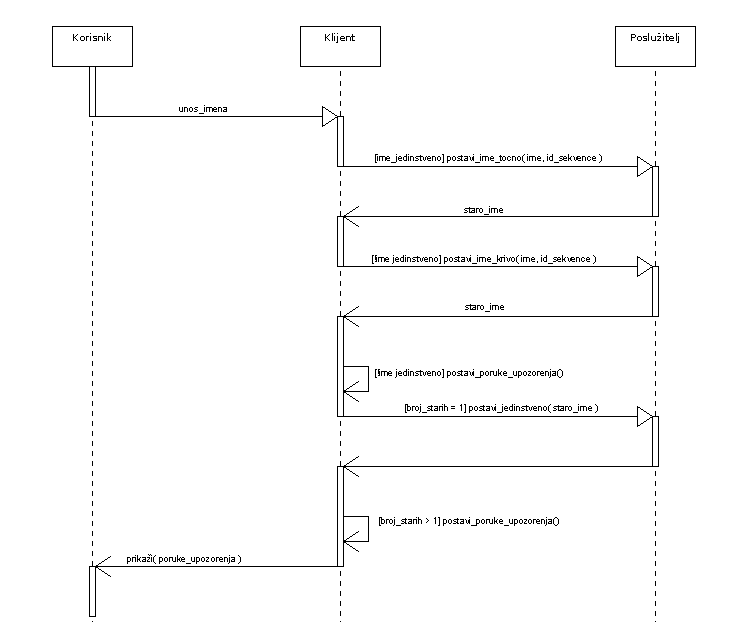
\includegraphics[width=5.3in]{figures/Unos_imena.png}
\caption{UML sekvencijski dijagram koji prikazuje slijed operacija prilikom
unosa imena}
\label{fig:imena}
\end{figure}

Obrada i spremanje podataka prilikom unosa imena sekvence prikazani su
UML\footnote{Unified Modeling Language} sekvencijskim dijagramom na slici
\ref{fig:imena}. Obrada počinje automatski u pozadini netom nakon što se ime
unese. Klijent najprije pretražuje imena svih vidljivih sekvenci. Ukoliko je
postavljeno ime različito od svih drugih unesenih imena, AJAX pozivom se
dojavljuje poslužitelju da postavi uneseno ime za tu sekvencu. Nakon što postavi
ime, poslužitelj provjerava validnost svih podataka za danu sekvencu te vraća
staro ime koje je bilo pridruženo sekvenci. Klijent briše eventualne poruke
upozorenja za danu sekvencu jer je ime jedinstveno. U slučaju da uneseno ime
nije jedinstveno, AJAX-om se dojavljuje poslužitelju uneseno ime uz naznaku da
je krivo. Svim sekvencama sa unesenim imenom poslužitelj miče zastavicu da su
jedinstvena te pokreće validciju njihovih podataka. Poslužitelj opet vraća staro
ime sekvence sa promijenjenim imenom. Također, u slučaju nejedinstvenog unesenog
imena, svim HTML elementima s istim imenom se pridružuje prikladna poruka
upozorenja. Nakon postavljanja imena na poslužitelju, klijent je dužan
provjeriti jesu li neka od jednakih imena na stranici trenutnim unosom
razriješena. Klijent dohvaća sve elemente s imenom jednakim starim imenom koje
je poslužitelj vratio. Ukoliko takvih nema, ništa se ne događa jer problema niti
nije bilo. Ako ih je više, na primjer 2, to znači da ih je prethodno bilo 3, ali
ta se imena i dalje trebaju razrješiti tako da im se poruke upozorenja ne miču.
Na poslijetku, ako je samo jedno ime pronađeno, njemu se brišu poruke upozorenja
te se AJAX-om dojavljuje poslužitelju da je ono od sada jedinstveno.

%todo -brisanje proteina sa stranice (sequence diagram)

%todo -unos FASTA (mislim da ne treba diagram) (text/file->iframe)

Validacija pojedine sekvence na poslužitelju postoji kako bi se svi podaci dane
sekvence provjerili jesu li uneseni i jesu li u dozvoljenom obliku kako bi se
jednostavnom provjerom zastavice 'OK' moglo ustvrditi može li dana sekvenca biti
proslijeđena u cjevovod. Prilikom validacije događaju se sljedeće provjere:

\begin{itemize}

\item je li sekvenca još aktivna?

\item je li uneseno ime jedinstveno? Ako nije, dozvoli iznimku za slučaj u kojem
ime nije uneseno, a postoji ime u FASTA zaglavlju unesene sekvence.

\item je li unesena sekvenca?

\end{itemize}

%todo -submit i nastavak
